\section{Dualshock4 Treiber (Becker)}

\subsection{Übertragung}

\subsection{Version 1: eigens entwickelter Treiber}

\subsection{Version 2: Treiber basierend auf der Bluepad32 Bibliothek}

\subsection{Testing}

\section{Platformsteuerung (Becker)}

Die sogenannte Plattformsteuerung bezeichnet alle technischen Komponenten, die erforderlich sind, um die Plattform in ihrer Rotation, vertikalen Neigung sowie für die Abgabe eines Schusses zu steuern.

Für den genannten Zweck werden folgende Komponenten benötigt:

\begin{itemize}
    \item \textbf{Drehung und Neigung}
    \begin{itemize}
        \item zwei MG996R Servo Motoren
    \end{itemize}
    \item \textbf{Schussabgabe}
    \begin{itemize}
        \item zwei DC-Motoren (Flywheels)
        \item MG92B Servo Motor
    \end{itemize}
\end{itemize}

Da die maximale Ausgangsstärke eines GPIO-PINs des ESP-32 mit 40mA \cite[S.~53]{esp_datasheet} für die benötigten Motoren nicht ausreicht \cite{esp_platform_flywheel_motor,esp_platform_small_servo,esp_platform_servo}, wurden entsprechende Treiberbaords verwendet.
Konkret handelt es sich hierbei um ein PCA9685 PWM-Treiberboard für die Servomotoren und um per PWM steuerbare MOSFET-Module für die Flywheel-Motoren.

In der nachfolgenden Sektion wird der Entwurf des Codes erörtert, der erforderlich ist, um die genannten Teile anzusteuern.

\subsection{PWM Board Treiber (Becker)}

Das PCA9685 PWM-Treiberboard gestattet die gleichzeitige Anbindung von bis zu 16 Servomotoren.
Für die Stromversorgung steht ein Eingang mit einer Spannung von 5 Volt zur Verfügung.

Die Steuerung des Boards erfolgt durch das Schreiben verschiedener Werte in Konfigurationsregister, wobei das I²C-Protokoll zum Einsatz kommt. 
Der vorliegende Treiber wurde aus der Portierung eines bereits bestehenden Treibers \cite{esp_pca9685_blueprint} entwickelt, welcher in der Programmiersprache C++ implementiert war. 
Es wurde bewusst nur die Funktionalität portiert, die für den Umfang des Projekts von Relevanz war. 
Der Treiber umfasst demzufolge lediglich drei Funktionen:

\begin{itemize}
    \item \textbf{pca9685\_init}: Die Funktion erhält die gewünschte Konfiguration für das Board (beispielsweise die Bus-Adresse, die SDA- und SCL-Ports für den I²C-Bus) und initialisiert den I²C-Bus. 
    Im Anschluss registriert sie das Treiberboard und konfiguriert schließlich das Board mit der gewünschten PWM-Frequenz.
    \item \textbf{pca9685\_set\_pwm\_on\_off}: Mithilfe dieser Funktion besteht nun die Möglichkeit, einen Motor auf einem der 16 Kanäle zu steuern. 
    Der Parameter \textit{ON} ist eine 12-Bit Zahl beschreibt hierbei den Zeitpunkt in der Phase, an welchem der Ausgang auf 5 Volt geschalten wird. 
    \textit{OFF}, ebenfalls eine 12-Bit Zahl bezeichnet den Zeitpunkt, zu welchem der Ausgang wieder auf 0 Volt geregelt wird. 
    Eine grafische Veranschaulichung ist in Abbildung \ref{fig:esp_pca9685_on_off} ersichtlich. 
    Da für die Ansteuerung der Servo Motoren keine symmetrischen PWM-Signale benötigt werden, wird der Parameter \textit{ON} im Folgenden immer den Wert 0 annehmen.

    \begin{figure}[ht]
        \centering
        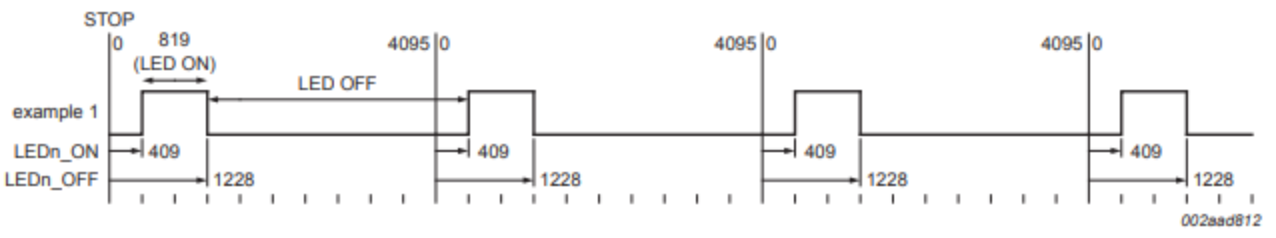
\includegraphics[width=\textwidth]{images/becker_esp_pca9685.png}
        \caption{Erklärung ON\slash OFF Parameter für PCA9685 aus \cite[S.~17]{esp_pca9685_datasheet}}
        \label{fig:esp_pca9685_on_off}
    \end{figure}

    \item \textbf{pca9685\_set\_off}: Mittels dieser Funktion kann das PWM-Signal auf einem bestimmten Kanal deaktiviert werden.
\end{itemize}

Auf Basis dieses Treiber wurden im nächsten Schritt zwei Interfaces programmiert: 
Einerseits das Interface zur Plattform-Kontrolle und andererseits das Interface zur Schusskontrolle, welches zusätzlich der Logik zur Ansteuerung der Flywheel-Motoren enthält.

\subsection{Ansteuerung der Servo-Motoren (Becker)}

Um nun die Platform sowohl mit manuellen Modus mit dem Dualshock4 Controller, als auch im semi-automatischen Modus mit künstlicher Intelligenz über MQTT präzise Steuern zu können,
wurde nun ein Interface entwickelt, welches die Ansteuerung eines Motors an eine gewisse Position erlaubt. 

Gearbeitet wird hier mit der Einheit Grad, ein Blick in das Datenblatt der Servo Motoren zeigt,
das durch die Einstellung der Duty-Cycle Länge des PWN-Signals eine Drehung auf eine gewisse Grad-Position erreicht wird. 
Im ersten Schritt wurden nun durch manuelles Testen die \textit{OFF} Werte für die Punkte \ang{-90} (max. Drehung nach links), \ang{0} und \ang{90} (max. Drehung nach rechts) ermittelt. 
Der Wert für die Drehung auf \ang{0} wird im Folgenden als $value_{zero}$ bezeichnet. 
Um nun den Zielwert $value_{off}$ für den \textit{OFF} Parameter des PWM Board Treibers zu berechnen, wird Formel \ref{eq:pwm_to_duty} verwendet:

\begin{gather}
    \begin{aligned}
    &\text{Sei } \theta \text{ der gewünschte Winkel,} \\
    &|\theta| = \text{Betrag von } \theta \\
    &n_3 = \left\lfloor \frac{|\theta|}{3} \right\rfloor \\
    &n_2 = |\theta| - n_3 \\
    &s = 2 \cdot n_2 + 3 \cdot n_3 \\
    &\tilde{s} =
    \begin{cases}
    s, & \theta > 0 \\
    -s, & \theta \leq 0
    \end{cases} \\
    &value_{off} = value_{zero} + \tilde{s}
    \end{aligned}
    \label{eq:pwm_to_duty}
\end{gather}



\subsection{Ansteuerung der Flywheel Motoren (Becker, Koch, Wohlrab)}

\section{Integration (Becker, Specht)}